\section{自治とは人間賛歌である:大学自治と学生自治へのエールを込めて}\label{sec:ningensanka}
\bunsekisha{文責}{Kyoto Science}

\begin{figure}[htbp]
  \begin{center}
    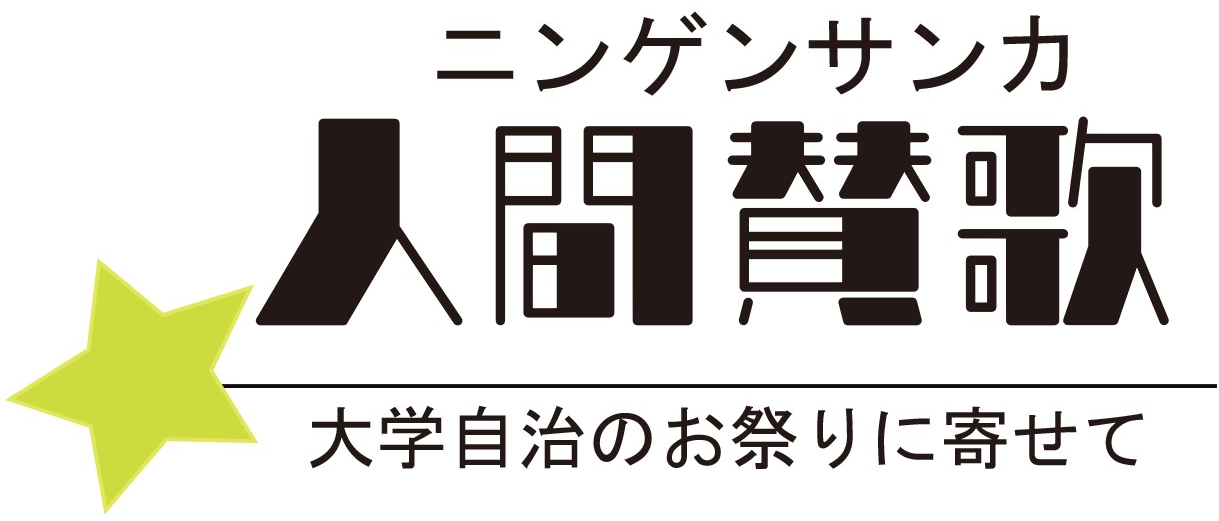
\includegraphics[width=0.7\textwidth]{gazo/ningensanka.png}
  \end{center}
\end{figure}

自治とは人間賛歌である、という話をします。

人間の力で現実を変えていけるという\hanten{人間賛歌が自治思想の根底にあります}。一方で、人間が現実の上にある、というこの人間賛歌は、実は未だ一般的ではありません。現実は不変の定数のように自分の力では変えられないものであり、変わるもの(変数)は自分の行動だけという諦めの感情が前提にあることが多いのです。

この世にオギャーと生まれてから、小中学校と学校社会に揉まれ、受験勉強や就職活動にあわあわとして、求められることは「ルールを理解してその中で行動すること」だけ、表のルールと裏のルールを理解して、不快感を与えることなく立ち回ることが“自主性”であると、うまくいかなければ偉い人・偉いルールを味方につけて他人の権力で殴ることが処世術であると、それを強いられてきた人も多いかもしれません。老若男女を問わずそうでしょう。出来れば権力を味方につけたいと、ルールの中で上位者になりたいと希い、さらなる権力者に一発逆転メシウマを望む人もいるでしょう。ただなぁ…。それ楽しいんか??

決められた\hanten{ルールや権力関係を絶対視する考え方は「ルールに基づき合理的に『君はもう、いらない』と見放されるリスク」と表裏一体}です。それにびくびくおどおどし、(まだ)見放されていないことに心の奥底で安堵しながら、不満を押し殺して生をやり過ごす。事情があるのもわかります。諦めていることもわかります。小市民的な生き方を全否定はしません。しかしながら、社会から「垢バン」されることに少しでも不安があるなら、全く違う道を---------諦めの中で小市民となることでもなく、自暴自棄になり暴れることでもない---------あなたに提示することが出来ます。それこそが人間賛歌であり、自治の精神なのです。

我々は、ここに第三の道を提示します。社会のルールを決める権力を自分たちの側に可能な限り引きずり下ろし、何をやっていいか、相手をどう受け止めるか、自分はどう生きるか、それら\hanten{すべてを自分たちで決める自治の道}を。すなわち、\hanten{令和の現代に送る人間賛歌}を提示します。

\subsection{自治とは何か、まず第一に決定権と決裁権を持つことです。}
社会や組織を車に例えると、自治は車検のようなものです。車はもしかするとオンボロの軽自動車かもしれませんし、性能マシマシのF1マシンかもしれません。金と権力に任せて徹底的に居心地よくしたリムジンかもしれません。しかしながら、車の性能や金額がいかなるものであれ、車検を通さない車はあり得ませんし、通さなければそのうち壊れいつか事故を起こします。そうなった時の責任は、車検を通さなかったドライバーにあるでしょう。

同様に、社会や組織が一部の有能なリーダーに頼って回っていたとしても、資本や権力を持つ集団が大きな顔をしていても、社会や組織の維持管理や運営を行いチェックするのは社会のドライバーたる我々です。そのための権限を担保すること、言い換えれば我々自身が社会の整備を行うための決定権を持つことが、自治活動の大きな意義の一つです。
 
\subsection{自治とは何か、第二には絶対の対等性です。}
自治空間は天下りのルールにより運営される空間ではなく、全員が実質的に対等な話し合いで運営されるべきです。(そうでないものは自治空間性が低いと思います。)これは全員がリソースを出すことにより全員が主権を持つここと、主権を全員が主張できる開放性によるものです。これにより人間を極力排除しない空間ができ、その安心感のなかで好きなことをできます。いつか一方的に追い出されるんじゃないか、クビになるんじゃないか、みんながさっと離れるんじゃないか。理想的な自治空間では、こうした不安は全て消えます。全員が自治空間のリソースとなることにより主権を得るからです。
 
\subsection{自治とは何か、第三にはしたいことをできる空間です。}
自分たちのルールを---------スポンサーや外部機関によらず---------自分たちで決めることで、本当に必要なこと、本当にやりたかったこと、本当にやりたくないこと。こうした構成員の意思を尊重し、現実に移すことが出来る空間です。あなたたちのことはあなたたちが決めていい。但し、自治空間のメリットを享受したひとは、自治空間の維持発展や拡大、自治空間同士の連携に可能な範囲で協力してほしいなという思いはあります。自分たちがリソースになることで、自分たちがしたいことをできる空間を手作りする。これが1つの肝なのです。
 
\begin{center}
  \hanten{では自治空間をどうやって作ればいいのか。}

  \hanten{その実験場こそが大学自治であり、学生自治が行われている、今、ここです。}
\end{center}

{\Large
  全ての自治空間に住む人よ。

  自治とは何か。

  見せて、

  診せて、

  魅せていきましょう。
}
 	
\emphbf{自治空間を社会に見せていこう。みんなに診させて体得してもらおう。人間賛歌にすべてを惹きつけよう}。日々悩み、お祭りで喜び、実力闘争で人事権と決裁権を維持しよう、ヒトとヒトとの交渉で社会を手作りで作り上げよう。手作りのための道具と技術を皆に渡そう。大学を超えて自治を社会に染み出させよう。それこそが社会と組織に人間賛歌を取り戻すための道だ。老若男女が共に生きる策だ。尊重と合意を基盤とした生への道だ。

諦観でも冷笑でも自暴自棄でもないこれこそが、そう、希望を現実に取り戻すための、人間賛歌の表れなのだ。

\emphbf{今この瞬間から、あなたも自治の仲間だ。}

\emphbf{共に、生きましょう。}

\emphbf{溢れんばかりの人間賛歌を浴びながら}


(「千万遍石垣」掲載:\url{https://senmanben.com/20221125/5447/})
